\documentclass[a4paper,num-refs]{oup-contemporary}

\title{Simulators on IBM Quantum Lab}
\author{Qiskit}
\authnote{\href{https://qiskit.org/documentation/stable/0.24/tutorials/simulators/1_aer_provider.html}{https://qiskit.org/documentation/stable/0.24/tutorials/simulators/1\_aer\_provider.html}}

\begin{document}
\begin{frontmatter}
\maketitle
\end{frontmatter}

\section{Abstract}
This notebook shows how to import Qiskit Aer simulator backends and use them to execute ideal (noise free) Qiskit Terra circuits.

\section{Qiskit Aer simulator backends}

Qiskit Aer currently includes three high performance simulator backends:
\begin{itemize}
    \item \verb|QasmSimulator|: Allows ideal and noisy multi-shot execution of qiskit circuits and returns counts or memory 
    \item \verb|StatevectorSimulator|: Allows ideal single-shot execution of qiskit circuits and returns the final statevector of the simulator after application.
    \item \verb|UnitarySimulator|: Allows ideal single-shot execution of qiskit circuits and returns the final unitary matrix of the circuit itself. Note that the circuit cannot contain measure or reset operations for this backend.
\end{itemize}

These backends are found in the Aer provider with the names \verb|qasm_simulator|, \verb|statevector_simulator| and \verb|unitary_simulator|, respectively and they can also be directly imported from \verb|qiskit.providers.aer|.

\subsection{QasmSimulator}
The \verb|QasmSimulator| backend is designed to mimic an actual device. It executes a Qiskit \verb|QuantumCircuit| and returns a count dictionary containing the final values of any classical registers in the circuit. The circuit may contain gates, measurements, resets, conditionals, and other advanced simulator options.

\subsection{StatevectorSimulator}

The \verb|StatevectorSimulator| executes a single shot of a Qiskit \verb|QuantumCircuit| and returns the final quantum statevector of the simulation. The circuit may contain gates, measurements, resets, and conditional operations.

\subsection{UnitarySimulator}

The \verb|UnitarySimulator| constructs the unitary matrix for a Qiskit \verb|QuantumCircuit| by applying each gate matrix to an identity matrix. The circuit may only contain gates, if it contains resets or measure operations an exception will be raised.

\section{Simulating a quantum circuit}
The basic operation define a quantum circuit we execute a simple 2-qubit Bell-state.

\begin{lstlisting}[language=Python]
circ = QuantumCircuit(2, 2)
circ.h(0)
circ.cx(0, 1)
\end{lstlisting}

\section{Simulation with a custom initial state}
We can begin with a custom initial statevector for the simulation.

\subsection{QasmSimulator and StatevectorSimulator}
The custom state may be set in the circuit using the \verb|initialize| method.

\begin{verbatim}
circ.initialize([1, 0, 0, 1] / np.sqrt(2), [0, 1])
\end{verbatim}

\subsection{UnitarySimulator}

We may also set an initial state for the \verb|UnitarySimulator|, however this state is an initial unitary matrix $U$, not a statevector and it will be used when the circuit is executed through the parameter \textit{initial\_unitary}.

\begin{lstlisting}[language=Python]
U = np.array([[ 1,  1,  0,  0],
              [ 0,  0,  1, -1],
              [ 0,  0,  1,  1],
              [ 1, -1,  0,  0]] / np.sqrt(2))
\end{lstlisting}

\begin{figure}[bt!] %% preferably at bottom or top of column
\centering
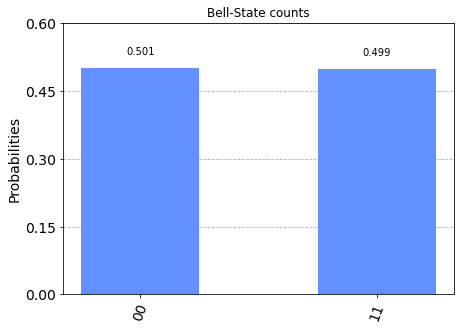
\includegraphics[width=\linewidth]{aer_provider_8_0.png}
\caption{Bell-State counts}\label{fig:bell-state-counts}
\end{figure}

\section{Select the simulator}
The simulator is chosen through the \verb|get\_backend| function from the \verb|Aer| provider. We can choose among the \verb|qasm_simulator|, \verb|statevector_simulator| and \verb|unitary_simulator| options.
\begin{verbatim}
simulator = Aer.get_backend('qasm_simulator')   
\end{verbatim}

\section{Execute the circuit and get results}

\subsection{QasmSimulator}

\subsubsection{Count outcomes}
The basic operation executes a quantum circuit and returns a counts dictionary of measurement outcomes (Fig.~\ref{fig:bell-state-counts}).
\begin{lstlisting}[language=Python]
circ.measure([0,1], [0,1])
result = execute(circ, simulator).result()
counts = result.get_counts(circ)
plot_histogram(counts, title='Bell-State counts') 
\end{lstlisting}


The \verb|QasmSimulator| returning a list of measurement outcomes for each individual shot. This is enabled by setting the keyword argument \textit{memory=True} in the \verb|assemble| or \verb|execute| function.

\begin{lstlisting}[language=Python]
# Execute and get memory
circ.measure([0,1], [0,1])
exec = execute(circ, simulator, shots=10, memory=True)
memory = exec.result().get_memory(circ)
print(memory)
\end{lstlisting}

The result of the previous notebook is:
\begin{verbatim}
['11', '00', '11', '00', '00', '00', '00', '00', '00', '11']
\end{verbatim}

\subsection{StatevectorSimulator}

\subsubsection{Get the final state}

The basic operation return a final state (Fig.~\ref{fig:bell-state}).

\begin{lstlisting}[language=Python]
result = execute(circ, simulator).result()
statevector = result.get_statevector(circ)
plot_state_city(statevector, title='Bell state')
\end{lstlisting}

\begin{figure}[bt!] %% preferably at bottom or top of column
\centering
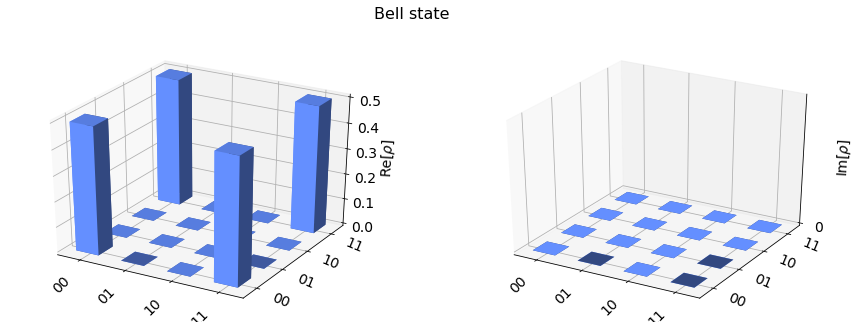
\includegraphics[width=\linewidth]{aer_provider_14_0.png}
\caption{Bell-State}\label{fig:bell-state}
\end{figure}

\subsubsection{Get the final state with measurement}

Note that if a circuit contains measure will be a conditional statevector after simulating wave-function collapse to the outcome of a measure (Fig. ~\ref{fig:bell-state-post-measurement}).

\begin{lstlisting}[language=Python]
circ.measure([0,1], [0,1])
result = execute(circ, simulator).result()
sv = result.get_statevector(circ)
plot_state_city(sv, title='Bell state measurement')
\end{lstlisting}

\begin{figure}[bt!] %% preferably at bottom or top of column
\centering
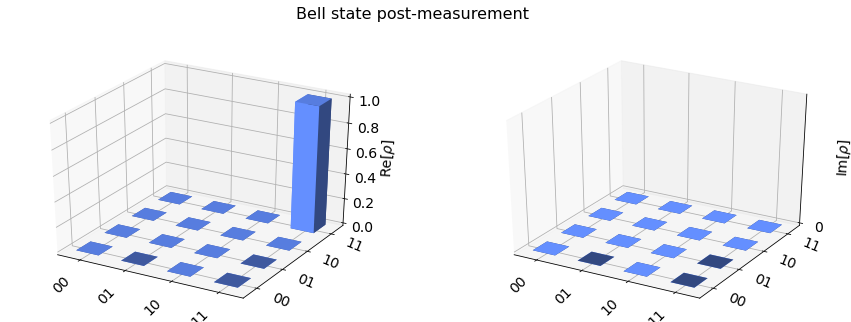
\includegraphics[width=\linewidth]{aer_provider_16_0.png}
\caption{Bell-State post-measurement}\label{fig:bell-state-post-measurement}
\end{figure}

\subsection{UnitarySimulator}
The basic operation return the unitary matrix corresponding to the circuit.

\begin{lstlisting}[language=Python]
result = execute(circ, simulator).result()
unitary = result.get_unitary(circ)
print("Circuit unitary:\n", unitary)
\end{lstlisting}

The result is:

\begin{verbatim}
Circuit unitary:
 [[ 0.70710678+0.00000000e+00j  0.70710678-8.65956056e-17j
    0.        +0.00000000e+00j  0.        +0.00000000e+00j]
  [ 0.        +0.00000000e+00j  0.        +0.00000000e+00j
    0.70710678+0.00000000e+00j -0.70710678+8.65956056e-17j]
  [ 0.        +0.00000000e+00j  0.        +0.00000000e+00j
    0.70710678+0.00000000e+00j  0.70710678-8.65956056e-17j]
  [ 0.70710678+0.00000000e+00j -0.70710678+8.65956056e-17j
    0.        +0.00000000e+00j  0.        +0.00000000e+00j]]
\end{verbatim}

\end{document}
